\documentclass[letterpaper,superscriptaddress,showkeys,longbibliography,10pt]{revtex4-1}\usepackage{graphicx, color}
%% maxwidth is the original width if it is less than linewidth
%% otherwise use linewidth (to make sure the graphics do not exceed the margin)
\makeatletter
\def\maxwidth{ %
  \ifdim\Gin@nat@width>\linewidth
    \linewidth
  \else
    \Gin@nat@width
  \fi
}
\makeatother

\definecolor{fgcolor}{rgb}{0.2, 0.2, 0.2}
\newcommand{\hlnumber}[1]{\textcolor[rgb]{0,0,0}{#1}}%
\newcommand{\hlfunctioncall}[1]{\textcolor[rgb]{0.501960784313725,0,0.329411764705882}{\textbf{#1}}}%
\newcommand{\hlstring}[1]{\textcolor[rgb]{0.6,0.6,1}{#1}}%
\newcommand{\hlkeyword}[1]{\textcolor[rgb]{0,0,0}{\textbf{#1}}}%
\newcommand{\hlargument}[1]{\textcolor[rgb]{0.690196078431373,0.250980392156863,0.0196078431372549}{#1}}%
\newcommand{\hlcomment}[1]{\textcolor[rgb]{0.180392156862745,0.6,0.341176470588235}{#1}}%
\newcommand{\hlroxygencomment}[1]{\textcolor[rgb]{0.43921568627451,0.47843137254902,0.701960784313725}{#1}}%
\newcommand{\hlformalargs}[1]{\textcolor[rgb]{0.690196078431373,0.250980392156863,0.0196078431372549}{#1}}%
\newcommand{\hleqformalargs}[1]{\textcolor[rgb]{0.690196078431373,0.250980392156863,0.0196078431372549}{#1}}%
\newcommand{\hlassignement}[1]{\textcolor[rgb]{0,0,0}{\textbf{#1}}}%
\newcommand{\hlpackage}[1]{\textcolor[rgb]{0.588235294117647,0.709803921568627,0.145098039215686}{#1}}%
\newcommand{\hlslot}[1]{\textit{#1}}%
\newcommand{\hlsymbol}[1]{\textcolor[rgb]{0,0,0}{#1}}%
\newcommand{\hlprompt}[1]{\textcolor[rgb]{0.2,0.2,0.2}{#1}}%

\usepackage{framed}
\makeatletter
\newenvironment{kframe}{%
 \def\at@end@of@kframe{}%
 \ifinner\ifhmode%
  \def\at@end@of@kframe{\end{minipage}}%
  \begin{minipage}{\columnwidth}%
 \fi\fi%
 \def\FrameCommand##1{\hskip\@totalleftmargin \hskip-\fboxsep
 \colorbox{shadecolor}{##1}\hskip-\fboxsep
     % There is no \\@totalrightmargin, so:
     \hskip-\linewidth \hskip-\@totalleftmargin \hskip\columnwidth}%
 \MakeFramed {\advance\hsize-\width
   \@totalleftmargin\z@ \linewidth\hsize
   \@setminipage}}%
 {\par\unskip\endMakeFramed%
 \at@end@of@kframe}
\makeatother

\definecolor{shadecolor}{rgb}{.97, .97, .97}
\definecolor{messagecolor}{rgb}{0, 0, 0}
\definecolor{warningcolor}{rgb}{1, 0, 1}
\definecolor{errorcolor}{rgb}{1, 0, 0}
\newenvironment{knitrout}{}{} % an empty environment to be redefined in TeX

\usepackage{alltt}
\usepackage[utf8]{inputenc}
\usepackage{color,dcolumn,graphicx,hyperref}
\usepackage[titletoc, title]{appendix}
\hypersetup
{
colorlinks = true, linkcolor = blue, citecolor = blue, urlcolor = blue,
}
\IfFileExists{upquote.sty}{\usepackage{upquote}}{}

\begin{document}



\begin{appendices}

\section{A complete reproducible workflow, from a species list to a phylogeny, and distribution map.} 

If you aren't familiar with a complete workflow in R, it may be difficult to visualize the process. In R, everything is programmatic, so the whole workflow can be in one place, and be repeated whenever necessary. The following is a workflow for taxize, going from a species list to a phylogeny. 

First, install taxize

\begin{knitrout}
\definecolor{shadecolor}{rgb}{0.969, 0.969, 0.969}\color{fgcolor}\begin{kframe}
\begin{alltt}
\hlfunctioncall{install.packages}(\hlstring{"taxize"})
\end{alltt}
\end{kframe}
\end{knitrout}


Then load it into R

\begin{knitrout}
\definecolor{shadecolor}{rgb}{0.969, 0.969, 0.969}\color{fgcolor}\begin{kframe}
\begin{alltt}
\hlfunctioncall{library}(taxize)
\end{alltt}
\end{kframe}
\end{knitrout}


Most of us will start out with a species list, something like the one below. Note that each of the names is spelled incorrectly.

\begin{knitrout}
\definecolor{shadecolor}{rgb}{0.969, 0.969, 0.969}\color{fgcolor}\begin{kframe}
\begin{alltt}
splist <- \hlfunctioncall{c}(\hlstring{"Helanthus annuus"}, \hlstring{"Pinos contorta"}, \hlstring{"Collomia grandiflorra"}, \hlstring{"Abies magnificaa"}, 
    \hlstring{"Rosa california"}, \hlstring{"Datura wrighti"}, \hlstring{"Mimulus bicolour"}, \hlstring{"Nicotiana glauca"}, 
    \hlstring{"Maddia sativa"}, \hlstring{"Bartlettia scapposa"})
\end{alltt}
\end{kframe}
\end{knitrout}


There are many ways to resolve taxonomic names in taxize. Of course, the ideal name resolver will do the work behind the scenes for you so that you don't have to do things like fuzzy matching. There are a few services in taxize like this we can choose from: the Global Names Resolver service from EOL (see function \emph{gnr\_resolve}) and the Taxonomic Name Resolution Service from iPlant (see function \emph{tnrs}). In this case let's use the function \emph{tnrs}. 

\begin{knitrout}
\definecolor{shadecolor}{rgb}{0.969, 0.969, 0.969}\color{fgcolor}\begin{kframe}
\begin{alltt}
\hlcomment{# The tnrs function accepts a vector of 1 or more}
splist_tnrs <- \hlfunctioncall{tnrs}(query = splist, getpost = \hlstring{"POST"}, source_ = \hlstring{"iPlant_TNRS"})

\hlcomment{# Remove some fields}
(splist_tnrs <- splist_tnrs[, !\hlfunctioncall{names}(splist_tnrs) %in% \hlfunctioncall{c}(\hlstring{"matchedName"}, \hlstring{"annotations"}, 
    \hlstring{"uri"})])
\end{alltt}
\begin{verbatim}
           submittedName         acceptedName    sourceId score
3       Helanthus annuus    Helianthus annuus iPlant_TNRS  0.98
1         Pinos contorta       Pinus contorta iPlant_TNRS  0.96
4  Collomia grandiflorra Collomia grandiflora iPlant_TNRS  0.99
5       Abies magnificaa      Abies magnifica iPlant_TNRS  0.98
10       Rosa california     Rosa californica iPlant_TNRS  0.99
9         Datura wrighti      Datura wrightii iPlant_TNRS  0.98
7       Mimulus bicolour      Mimulus bicolor iPlant_TNRS  0.98
8       Nicotiana glauca     Nicotiana glauca iPlant_TNRS  1.00
6          Maddia sativa         Madia sativa iPlant_TNRS  0.97
2    Bartlettia scapposa   Bartlettia scaposa iPlant_TNRS  0.98
\end{verbatim}
\begin{alltt}

\hlcomment{# Note the scores. They suggest that there were no perfect matches, but}
\hlcomment{# they were all very close, ranging from 0.77 to 0.99 (1 is the highest).}
\hlcomment{# Let's assume the names in the 'acceptedName' column are correct (and}
\hlcomment{# they should be).}

\hlcomment{# So here's our updated species list}
(splist <- \hlfunctioncall{as.character}(splist_tnrs$acceptedName))
\end{alltt}
\begin{verbatim}
 [1] "Helianthus annuus"    "Pinus contorta"       "Collomia grandiflora"
 [4] "Abies magnifica"      "Rosa californica"     "Datura wrightii"     
 [7] "Mimulus bicolor"      "Nicotiana glauca"     "Madia sativa"        
[10] "Bartlettia scaposa"  
\end{verbatim}
\end{kframe}
\end{knitrout}


Another thing we may want to do is collect common names for our taxa. 

\begin{knitrout}
\definecolor{shadecolor}{rgb}{0.969, 0.969, 0.969}\color{fgcolor}\begin{kframe}
\begin{alltt}
tsns <- \hlfunctioncall{get_tsn}(searchterm = splist, searchtype = \hlstring{"sciname"}, verbose = FALSE)
comnames <- \hlfunctioncall{lapply}(tsns, getcommonnamesfromtsn)

\hlcomment{# Unfortunately, common names are not standardized like species names, so}
\hlcomment{# there are multiple common names for each taxon}
\hlfunctioncall{sapply}(comnames, length)
\end{alltt}
\begin{verbatim}
 [1] 3 3 3 3 3 3 3 3 3 3
\end{verbatim}
\begin{alltt}

\hlcomment{# So let's just take the first common name for each species}
comnames_vec <- \hlfunctioncall{do.call}(c, \hlfunctioncall{lapply}(comnames, \hlfunctioncall{function}(x) \hlfunctioncall{as.character}(x[1, \hlstring{"comname"}])))

\hlcomment{# And we can make a data.frame of our scientific and common names}
(allnames <- \hlfunctioncall{data.frame}(spname = splist, comname = comnames_vec))
\end{alltt}
\begin{verbatim}
                 spname                       comname
1     Helianthus annuus              common sunflower
2        Pinus contorta                lodgepole pine
3  Collomia grandiflora        largeflowered collomia
4       Abies magnifica                    golden fir
5      Rosa californica           California wildrose
6       Datura wrightii            sacred thorn-apple
7       Mimulus bicolor yellow and white monkeyflower
8      Nicotiana glauca                  tree tobacco
9          Madia sativa                 coast tarweed
10   Bartlettia scaposa                Bartlett daisy
\end{verbatim}
\end{kframe}
\end{knitrout}


Another common task is getting the taxonomic tree upstream from your study taxa. We often know what family or order our taxa are in, but it we often don't know the tribes, subclasses, and superfamilies. taxize provides many avenues to getting classifications. Two of them are accessible via a single function (\emph{classification}): the Integrated Taxonomic Information System (ITIS) and National Center for Biotechnology Information (NCBI); and via the Catalogue of Life (see function \emph{col\_classification}):

\begin{knitrout}
\definecolor{shadecolor}{rgb}{0.969, 0.969, 0.969}\color{fgcolor}\begin{kframe}
\begin{alltt}
\hlcomment{# As we already have Taxonomic Serial Numbers from ITIS, let's just get}
\hlcomment{# classifications from ITIS. Note that we could use uBio instead.}
class_list <- \hlfunctioncall{classification}(tsns)
\hlfunctioncall{sapply}(class_list, nrow)
\end{alltt}
\begin{verbatim}
 [1] 12 11 12 11 12 12 12 12 12 12
\end{verbatim}
\begin{alltt}

\hlcomment{# And we can attach these names to our allnames data.frame}
\hlfunctioncall{library}(plyr)
gethiernames <- \hlfunctioncall{function}(x) \{
    temp <- x[, \hlfunctioncall{c}(\hlstring{"rankName"}, \hlstring{"taxonName"})]
    values <- \hlfunctioncall{data.frame}(\hlfunctioncall{t}(temp[, 2]))
    \hlfunctioncall{names}(values) <- temp[, 1]
    \hlfunctioncall{return}(values)
\}
class_df <- \hlfunctioncall{ldply}(class_list, gethiernames)
allnames_df <- \hlfunctioncall{merge}(allnames, class_df, by.x = \hlstring{"spname"}, by.y = \hlstring{"Species"})

\hlcomment{# Now that we have allnames_df, we can start to see some relationships}
\hlcomment{# among species simply by their shared taxonomic names}
allnames_df[1:2, ]
\end{alltt}
\begin{verbatim}
              spname        comname Kingdom     Subkingdom Infrakingdom
1    Abies magnifica     golden fir Plantae Viridaeplantae Streptophyta
2 Bartlettia scaposa Bartlett daisy Plantae Viridaeplantae Streptophyta
      Division     Subdivision Infradivision         Class Superorder
1 Tracheophyta Spermatophytina  Gymnospermae     Pinopsida       <NA>
2 Tracheophyta Spermatophytina  Angiospermae Magnoliopsida  Asteranae
      Order     Family      Genus
1   Pinales   Pinaceae      Abies
2 Asterales Asteraceae Bartlettia
\end{verbatim}
\begin{alltt}

\hlcomment{# Ah, so Abies and Bartlettia are in different infradivisions, but share}
\hlcomment{# taxonomic names above that point.}
\end{alltt}
\end{kframe}
\end{knitrout}


However, taxonomy can only get you so far. Shared ancestry can be reconstructed from molecular data, and phylogenies created. Phylomatic is a web service with an API that we can use to get a phylogeny. 

\begin{figure}[!h] 
\centering 
\begin{knitrout}
\definecolor{shadecolor}{rgb}{0.969, 0.969, 0.969}\color{fgcolor}\begin{kframe}
\begin{alltt}
\hlcomment{# Fetch phylogeny from phylomatic}
phylogeny <- \hlfunctioncall{phylomatic_tree}(taxa = \hlfunctioncall{as.character}(allnames$spname), taxnames = TRUE, 
    get = \hlstring{"POST"}, informat = \hlstring{"newick"}, method = \hlstring{"phylomatic"}, storedtree = \hlstring{"R20120829"}, 
    taxaformat = \hlstring{"slashpath"}, outformat = \hlstring{"newick"}, clean = \hlstring{"true"}, parallel = TRUE)
\hlcomment{# Format teeth-labels}
phylogeny$tip.label <- \hlfunctioncall{capwords}(phylogeny$tip.label, onlyfirst = TRUE)
\hlcomment{# plot phylogeny}
\hlfunctioncall{plot}(phylogeny)
\end{alltt}
\end{kframe}

{\centering 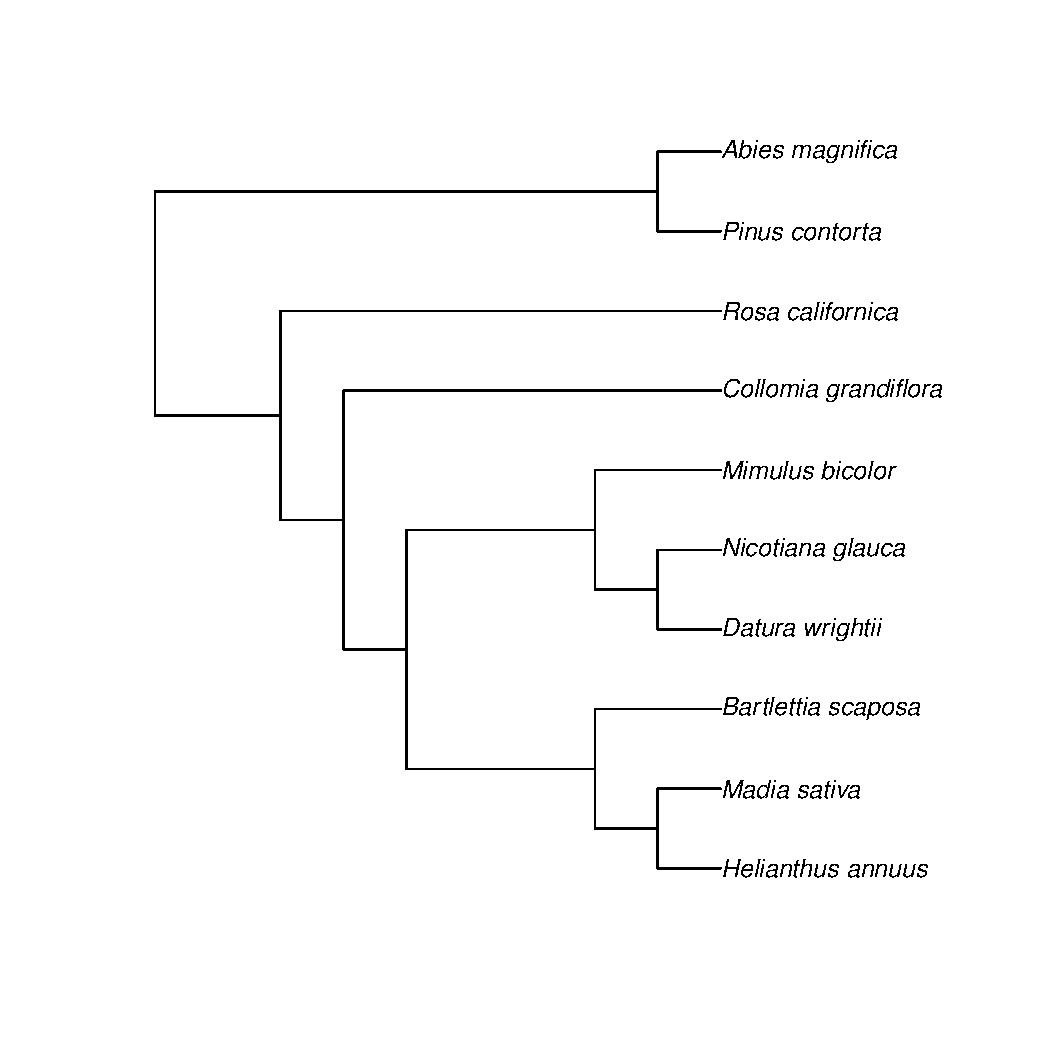
\includegraphics[width=4in,height=4in]{figure/phylogeny} 

}



\end{knitrout}

\caption{a phylogeny...} 
\end{figure} 

Using the species list, with the corrected names, we can now search for occurrence data. The Global Biodiversity Information Facility (GBIF) has the largest collection of records data, and has a  API that we can interact with programmatically from R. First, we need to install rgbif.

\begin{knitrout}
\definecolor{shadecolor}{rgb}{0.969, 0.969, 0.969}\color{fgcolor}\begin{kframe}
\begin{alltt}
\hlcomment{# Install rgbif from github.com}
\hlfunctioncall{install.packages}(\hlstring{"devtools"})
\hlfunctioncall{library}(devtools)
\hlfunctioncall{install_github}(\hlstring{"rgbif"}, \hlstring{"ropensci"})
\end{alltt}
\end{kframe}
\end{knitrout}


Now we can search for occurrences for our species list and make a map.


\begin{knitrout}
\definecolor{shadecolor}{rgb}{0.969, 0.969, 0.969}\color{fgcolor}\begin{kframe}
\begin{alltt}
\hlfunctioncall{library}(rgbif)
\hlfunctioncall{library}(ggplot2)

\hlcomment{# get occurences}
occurr_list <- \hlfunctioncall{occurrencelist_many}(\hlfunctioncall{as.character}(allnames$spname), coordinatestatus = TRUE, 
    maxresults = 100, removeZeros = TRUE, fixnames = \hlstring{"changealltorig"})

\hlcomment{# Make a map}
p <- \hlfunctioncall{gbifmap}(occurr_list) + \hlfunctioncall{guides}(col = \hlfunctioncall{guide_legend}(title = \hlstring{""}, nrow = 3, 
    byrow = TRUE)) + \hlfunctioncall{theme}(legend.position = \hlstring{"bottom"}, legend.key = \hlfunctioncall{element_blank}()) + 
    \hlfunctioncall{coord_equal}()
p
\end{alltt}
\end{kframe}\begin{figure}[h]


{\centering 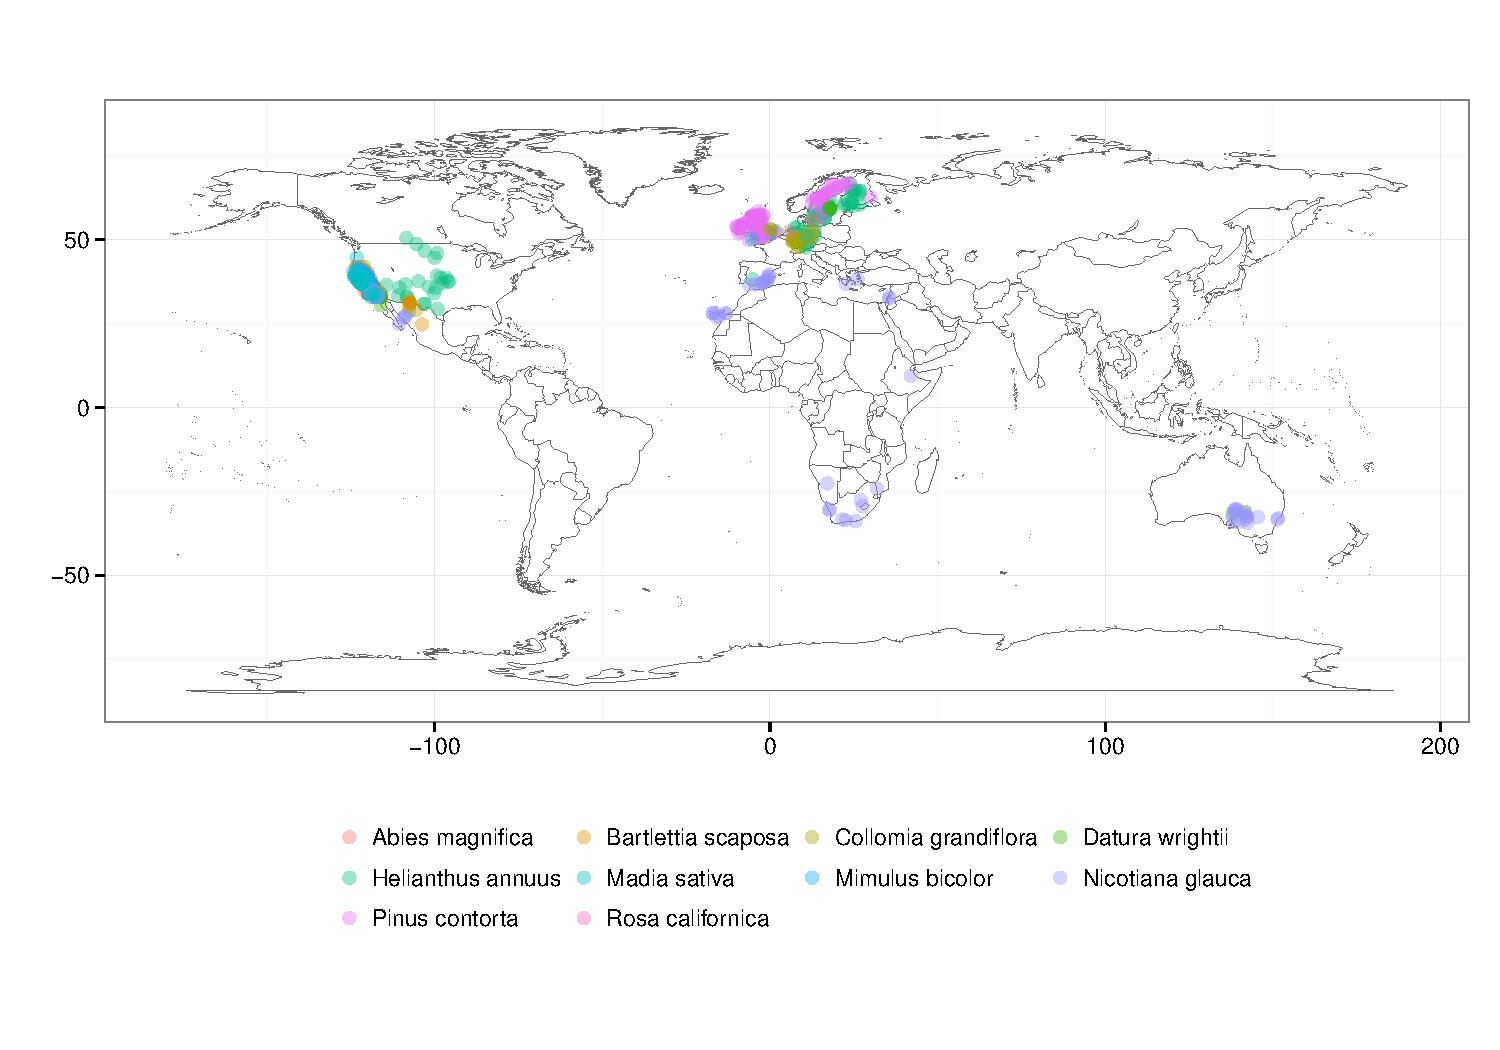
\includegraphics[width=.9\textwidth]{figure/plot_map} 

}

\caption[A map]{A map\label{fig:mapplot_map}}
\end{figure}


\end{knitrout}



\newpage

\section{Matching species tables with different taxonomic resolution} 

Trait-based approaches are a promising tool in ecology. Unlike taxonomy-based methods, traits may not be constrained to biogeographic boundaries \citep{baird_toward_2011} and have potential to disentangle the effects of multiple stressors \citep{statzner_can_2010}. 

To analyse trait-composition abundance data must be matched with trait databases like \citet{usseglio-polatera_biological_2000}. However these two datatables may contain species information on different taxonomic levels and perhabs data must be aggregated to a joint taxomic level.

taxize can help in this data-cleaning step, providing a reproducible workflow. Here we illustrate this on a small fictitious example.

Suppose we have fuzzy coded trait table with 2 traits with 3 respectively 2 modalities:
\begin{knitrout}
\definecolor{shadecolor}{rgb}{0.969, 0.969, 0.969}\color{fgcolor}\begin{kframe}
\begin{alltt}
(traits <- \hlfunctioncall{read.table}(header = TRUE, sep = \hlstring{';'}, stringsAsFactors=FALSE, 
                      text = 'taxon;T1M1;T1M2;T1M3;T2M1;T2M2
Gammarus sp.;0;0;3;1;3
Potamopyrgus antipodarum;1;0;3;1;3
Coenagrion sp.;3;0;1;3;1
Enallagma cyathigerum;0;3;1;0;3
Erythromma sp.;0;0;3;3;1
Baetis sp.;0;0;0;0;0
'))
\end{alltt}
\begin{verbatim}
                     taxon T1M1 T1M2 T1M3 T2M1 T2M2
1             Gammarus sp.    0    0    3    1    3
2 Potamopyrgus antipodarum    1    0    3    1    3
3           Coenagrion sp.    3    0    1    3    1
4    Enallagma cyathigerum    0    3    1    0    3
5           Erythromma sp.    0    0    3    3    1
6               Baetis sp.    0    0    0    0    0
\end{verbatim}
\end{kframe}
\end{knitrout}


And want to match this to a table with abundances:
\begin{knitrout}
\definecolor{shadecolor}{rgb}{0.969, 0.969, 0.969}\color{fgcolor}\begin{kframe}
\begin{alltt}
(abundances <- \hlfunctioncall{read.table}(header = TRUE, sep = \hlstring{';'}, stringsAsFactors=FALSE, 
                          text = 'taxon;abundance;sample
Gammarus roeseli;5;1
Gammarus roeseli;6;2
Gammarus tigrinus;7;1
Gammarus tigrinus;8;2
Coenagrionidae;10;1
Coenagrionidae;6;2
Potamopyrgus antipodarum;10;1
xxxxx;10;2
'))
\end{alltt}
\begin{verbatim}
                     taxon abundance sample
1         Gammarus roeseli         5      1
2         Gammarus roeseli         6      2
3        Gammarus tigrinus         7      1
4        Gammarus tigrinus         8      2
5           Coenagrionidae        10      1
6           Coenagrionidae         6      2
7 Potamopyrgus antipodarum        10      1
8                    xxxxx        10      2
\end{verbatim}
\end{kframe}
\end{knitrout}



First we do some basic data-cleaning and create a lookup-table, that will link taxa in trait table with the abundance table.
\begin{knitrout}
\definecolor{shadecolor}{rgb}{0.969, 0.969, 0.969}\color{fgcolor}\begin{kframe}
\begin{alltt}
\hlcomment{# first we remove ' sp.' from out trait table:}
traits$taxon_cleaned <- \hlfunctioncall{tolower}(\hlfunctioncall{gsub}(\hlstring{" sp."}, \hlstring{""}, traits$taxon))

\hlcomment{# since abundance tables can be very long with repeating taxa, we look}
\hlcomment{# only at unique taxon names This will be a lookup-table linking taxon}
\hlcomment{# names between both tables}
lookup <- \hlfunctioncall{data.frame}(taxon = \hlfunctioncall{tolower}(\hlfunctioncall{unique}(abundances$taxon)), stringsAsFactors = FALSE)
\end{alltt}
\end{kframe}
\end{knitrout}


The we query the taxonomic hierarchy for both tables, this will be the backbone of this procedure:
\begin{knitrout}
\definecolor{shadecolor}{rgb}{0.969, 0.969, 0.969}\color{fgcolor}\begin{kframe}
\begin{alltt}
\hlfunctioncall{require}(taxize)
traits_classi <- \hlfunctioncall{classification}(\hlfunctioncall{get_uid}(traits$taxon_cleaned))
lookup_classi <- \hlfunctioncall{classification}(\hlfunctioncall{get_uid}(lookup$taxon))
\end{alltt}
\end{kframe}
\end{knitrout}


First we look if we can find any direct matches between taxon names:
\begin{knitrout}
\definecolor{shadecolor}{rgb}{0.969, 0.969, 0.969}\color{fgcolor}\begin{kframe}
\begin{alltt}
\hlcomment{# first search for direct matches}
direct <- \hlfunctioncall{match}(lookup$taxon, traits$taxon_cleaned)
\hlcomment{# and add the matched name to our lookup table}
lookup$traits <- \hlfunctioncall{tolower}(traits$taxon[direct])
lookup$match <- \hlfunctioncall{ifelse}(!\hlfunctioncall{is.na}(direct), \hlstring{"direct"}, NA)
lookup
\end{alltt}
\begin{verbatim}
                     taxon                   traits  match
1         gammarus roeseli                     <NA>   <NA>
2        gammarus tigrinus                     <NA>   <NA>
3           coenagrionidae                     <NA>   <NA>
4 potamopyrgus antipodarum potamopyrgus antipodarum direct
5                    xxxxx                     <NA>   <NA>
\end{verbatim}
\end{kframe}
\end{knitrout}


We found a direct match - \emph{potamopyrgus antipodarum} - so nothing to do here.


Next we look for species which are on a higher taxonomic resolution than our trait table. 
For these species we will take directly the trait-data since no better information is available.

\begin{knitrout}
\definecolor{shadecolor}{rgb}{0.969, 0.969, 0.969}\color{fgcolor}\begin{kframe}
\begin{alltt}
\hlcomment{# look for cases where taxonomic resolution in abundance data is higher}
\hlcomment{# than in trait data: here we take the trait-values for the lower}
\hlcomment{# resolution}
\hlfunctioncall{for} (i in \hlfunctioncall{which}(\hlfunctioncall{is.na}(lookup$traits))) \{
    \hlfunctioncall{if} (\hlfunctioncall{is.data.frame}(lookup_classi[[i]])) \{
        matches <- \hlfunctioncall{tolower}(lookup_classi[[i]]$ScientificName) %in% traits$taxon_cleaned
        \hlfunctioncall{if} (\hlfunctioncall{any}(matches)) \{
            lookup$traits[i] <- \hlfunctioncall{tolower}(lookup_classi[[i]]$ScientificName[matches])
            lookup$match[i] <- lookup_classi[[i]]$Rank[matches]
        \}
    \}
\}
lookup
\end{alltt}
\begin{verbatim}
                     taxon                   traits  match
1         gammarus roeseli                 gammarus  genus
2        gammarus tigrinus                 gammarus  genus
3           coenagrionidae                     <NA>   <NA>
4 potamopyrgus antipodarum potamopyrgus antipodarum direct
5                    xxxxx                     <NA>   <NA>
\end{verbatim}
\end{kframe}
\end{knitrout}


So our abundance data has two Gammarus species, however trait data is only on genus level.


The next step is to search for species were we have to aggregate tait-data, since our abundance data is on a lower taxonomic level.
We are walking the taxomomic latter for the species in our trait-data upwards and search for matches with out abundance data. Since we'll have many taxa in the trait-data belonging to one taxon, we'll take the median modality scores as an approximation. Of course also other methods may be used here, e.g. weighting by genetic distance.


\begin{knitrout}
\definecolor{shadecolor}{rgb}{0.969, 0.969, 0.969}\color{fgcolor}\begin{kframe}
\begin{alltt}
\hlcomment{# look for cases taxonomic resolution in abundance data is lower than in}
\hlcomment{# trait data, here we need to aggregate the trait-values (eg. median value}
\hlcomment{# for modality)}

\hlfunctioncall{for} (i in \hlfunctioncall{which}(\hlfunctioncall{is.na}(lookup$traits))) \{
\hlcomment{    # find matches}
    agg <- \hlfunctioncall{sapply}(traits_classi, \hlfunctioncall{function}(x) \hlfunctioncall{any}(\hlfunctioncall{tolower}(x$ScientificName) %in% 
        lookup$taxon[i]))
    \hlfunctioncall{if} (\hlfunctioncall{sum}(agg) > 1) \{
\hlcomment{        # add taxon as aggregate to trait-table}
        traits <- \hlfunctioncall{rbind}(traits, \hlfunctioncall{c}(\hlfunctioncall{paste0}(lookup$taxon[i], \hlstring{"-aggregated"}), \hlfunctioncall{apply}(traits[agg, 
            2:6], 2, median), \hlfunctioncall{paste0}(lookup$taxon[i], \hlstring{"-aggregated"})))
\hlcomment{        # fill lookup table}
        lookup$traits[i] <- \hlfunctioncall{paste0}(lookup$taxon[i], \hlstring{"-aggregated"})
        lookup$match[i] <- \hlstring{"aggregated"}
    \}
\}
lookup
\end{alltt}
\begin{verbatim}
                     taxon                    traits      match
1         gammarus roeseli                  gammarus      genus
2        gammarus tigrinus                  gammarus      genus
3           coenagrionidae coenagrionidae-aggregated aggregated
4 potamopyrgus antipodarum  potamopyrgus antipodarum     direct
5                    xxxxx                      <NA>       <NA>
\end{verbatim}
\end{kframe}
\end{knitrout}


Finally we have only one taxon left - clearly an error. We remove this from our dataset:
\begin{knitrout}
\definecolor{shadecolor}{rgb}{0.969, 0.969, 0.969}\color{fgcolor}\begin{kframe}
\begin{alltt}
abundances <- abundances[!abundances$taxon == lookup$taxon[\hlfunctioncall{is.na}(lookup$traits)], 
    ]
\end{alltt}
\end{kframe}
\end{knitrout}



No we can create \emph{species x sites} and \emph{traits x species} matrices, which could be plugged into methods to analyse trait responses \citep{kleyer_assessing_2012}.


\begin{knitrout}
\definecolor{shadecolor}{rgb}{0.969, 0.969, 0.969}\color{fgcolor}\begin{kframe}
\begin{alltt}
\hlcomment{# species (as matched with trait table) by site matrix}
abundances$traits_taxa <- lookup$traits[\hlfunctioncall{match}(\hlfunctioncall{tolower}(abundances$taxon), lookup$taxon)]

\hlfunctioncall{require}(reshape2)
\hlcomment{# reshape data to long format and name rows by samples}
L <- \hlfunctioncall{dcast}(abundances, sample ~ traits_taxa, fun.aggregate = sum, value.var = \hlstring{"abundance"})
\hlfunctioncall{rownames}(L) <- L$sample
L$sample <- NULL
L
\end{alltt}
\begin{verbatim}
  coenagrionidae-aggregated gammarus potamopyrgus antipodarum
1                        10       12                       10
2                         6       14                        0
\end{verbatim}
\begin{alltt}

\hlcomment{# traits by species matrix}
Q <- traits[, 2:7][\hlfunctioncall{match}(\hlfunctioncall{names}(L), traits$taxon_cleaned), ]
\hlfunctioncall{rownames}(Q) <- Q$taxon_cleaned
Q$taxon_cleaned <- NULL
Q
\end{alltt}
\begin{verbatim}
                          T1M1 T1M2 T1M3 T2M1 T2M2
coenagrionidae-aggregated    0    0    1    3    1
gammarus                     0    0    3    1    3
potamopyrgus antipodarum     1    0    3    1    3
\end{verbatim}
\begin{alltt}

\hlcomment{# check}
\hlfunctioncall{all}(\hlfunctioncall{rownames}(Q) == \hlfunctioncall{colnames}(L))
\end{alltt}
\begin{verbatim}
[1] TRUE
\end{verbatim}
\end{kframe}
\end{knitrout}


This is just an example how taxonomic APIs (via taxize) could be used to search for matches up- and downwards the taxonomic ladder. We are looking forward to integrate the freshwaterecology.info database \citep{freshwaterecology} into taxize, which will facilitate trait-based analyses in R.

\end{appendices}

\bibliographystyle{eco_lett}
\bibliography{refs}

\end{document}
